\chapter{Collectivity in QCD}
\section{Conceptual Understanding of Flow}
\begin{figure}[h!]
\begin{center}
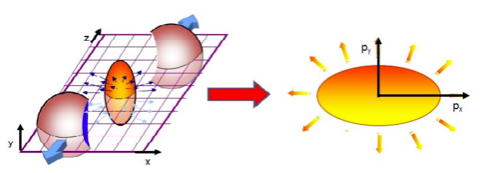
\includegraphics[width=0.45\linewidth]{figs/elliptical_flow_cartoon.png}
\caption{ TBA }
\end{center}
\end{figure}

\section{Mathematical Introduction}
A measurement of the azimuthal anisotropy is a way to quantify the extent of long-range angular correlation present in the medium evolution. One way to study the azimuthal anisotropy is to create a correlation function. The 2-particle correlation function method uses pairs of particles from the event in order to create a correlation function. For each each pair in an event, a $\Delta\phi$ value is obtained which makes up the signal $S(\Delta\phi,p_T)$. In order to correct for artificial correlations which would distort the distribution from detector effects or other sources, a mixed event background distribution $M(\Delta\phi,pT)$ is created. The correlation function can be defined as follows:

%\begin{equation}\label{eqn:corr_func}
%  C(\Delta,p_T) = \frac{S(\Delta\phi,p_T)}{M(\Delta\phi,p_T)}\frac{\int_{0}^{2\pi}M(\Delta\phi,p_T)d\Delta\phi)}{\int_0^{2\pi}S(\Delta\phi,p_T)d\Delta\phi)}
%\end{equation}

\begin{eqnarray}
  S(\Delta\phi,p_{T})=
  \frac{ d(w_{{\rm PMT}} N^{{\rm track}(p_{T}){\rm - PMT}}_{{\rm Same \; event}}) }{ d\Delta\phi}, & &
\label{eq31} \\
  C(\Delta\phi,p_{T}) =
          \frac{S(\Delta\phi,p_{T})}{M(\Delta\phi,p_{T})} \:
          \frac{\int_{0}^{2\pi} M(\Delta\phi,p_{T}) \, d\Delta\phi}{\int_{0}^{2\pi} S(\Delta\phi,p_{T}) \, d\Delta\phi}. & &
  \label{eq:def_corr_function}
\end{eqnarray}


Substantial variations in this $C(\Delta\phi,p_T)$ are usually seen as long-range angular correlations which can be attributed to collectivity.

In order to quantify the azimuthal anisotropy, $C(\Delta\phi,p_T)$ is Fourier transformed:
\begin{equation}\label{eqn:dndphi}
  C(\Delta\phi,p_T) \propto 1 + \sum_{n=1}2 v_{n}\cos(n[\phi(p_T)-\Psi_n]) 
\end{equation}

where $\Psi_n$ is the event plane angle, $\phi$ is the azimuth of tracks from the event, and $v_n$ are flow coefficients. The measured $v_n$ averaged over a single event is defined as:
\begin{equation}\label{eqn:vn}
  v_n = \frac{\langle\cos(n[\phi-\Psi_n])\rangle}{Res(\Psi_n)}
\end{equation}

where $Res(\Psi_n)$ is the event plane resolution for each event. $v_N$ are further averaged over each event.
\begin{equation}
\varepsilon_n = \frac{\sqrt{\langle r^2\cos (n\phi)\rangle ^2 + \langle r^2\sin (n\phi) \rangle ^2}}{\langle r^2 \rangle}
\end{equation}

\section{A Review of Flow Measurements in Heavy Ion Collisions}

\section{Collectivity in Small QCD Systems}
Small collision systems have been considered too small to create hot and dense matter. These systems were thought to be control experiments which could be used to measure cold nuclear matter effects. However, evidence of collectivity has recently been observed at RHIC in p+Au collisions at $\sqrt{s_{NN}}$ = 200 GeV in the most central collisions ~\cite{PhysRevLett.115.142301}. Although, the $p_T$ dependent $v_N$ has been measured, what has not been measured in these small systems is the degree to which $v_N$ changes a function of rapidity. This is a particularly interesting measurement to make in an asymmetric collision system such as p+Au.

Recent analyses of d+Au and HeAu collisions at $\sqrt{n}$ = 200 GeV~\cite{PhysRevLett.111.212301,Adare:2014keg,Adare:2015ctn,Adamczyk:2014fcx} at the Relativistic Heavy-Ion Collider (RHIC), and p+Pb at $\sqrt{n}$ = 5.02 TeV, and $p+p$ collisions at $\sqrt{n}$ = 2.76, 5.02, 7, and 13 TeV~\cite{alice_long_2013,atlas_observation_2012,cms_observation_2012,Khachatryan:2015lva,Aad:2015gqa,Khachatryan:2010gv,Khachatryan:2016txc} at the Large Hadron Collider (LHC) have demonstrated the existence of the same kind of azimuthal anisotropy signals commonly interpreted as evidence of collective behavior in larger systems. Notably, a feature known as \textit{the ridge} has been observed, consisting of a near-side (i.e., at small relative azimuth) enhancement in the long-range (i.e., at large relative pseudorapidity) azimuthal two-particle correlation. From these correlations, substantial elliptic ($v_2$), and triangular ($v_3$) flow coefficients have been measured in these systems.
\begin{figure}[h!]
\begin{center}
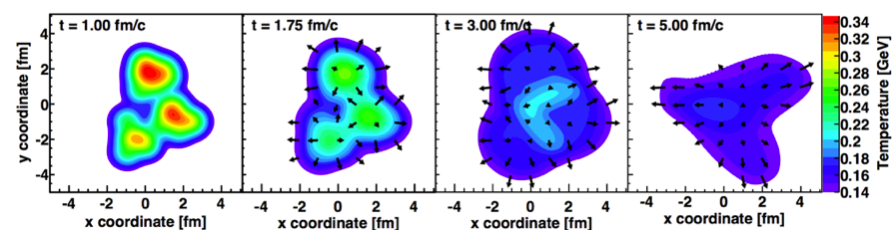
\includegraphics[width=0.45\linewidth]{figs/he3au_simulation.png}
\caption{ TBA }
\end{center}
\end{figure}


\subsection{Monte-Carlo Initial Condition Characterization}
\begin{figure}[h!]
\begin{center}
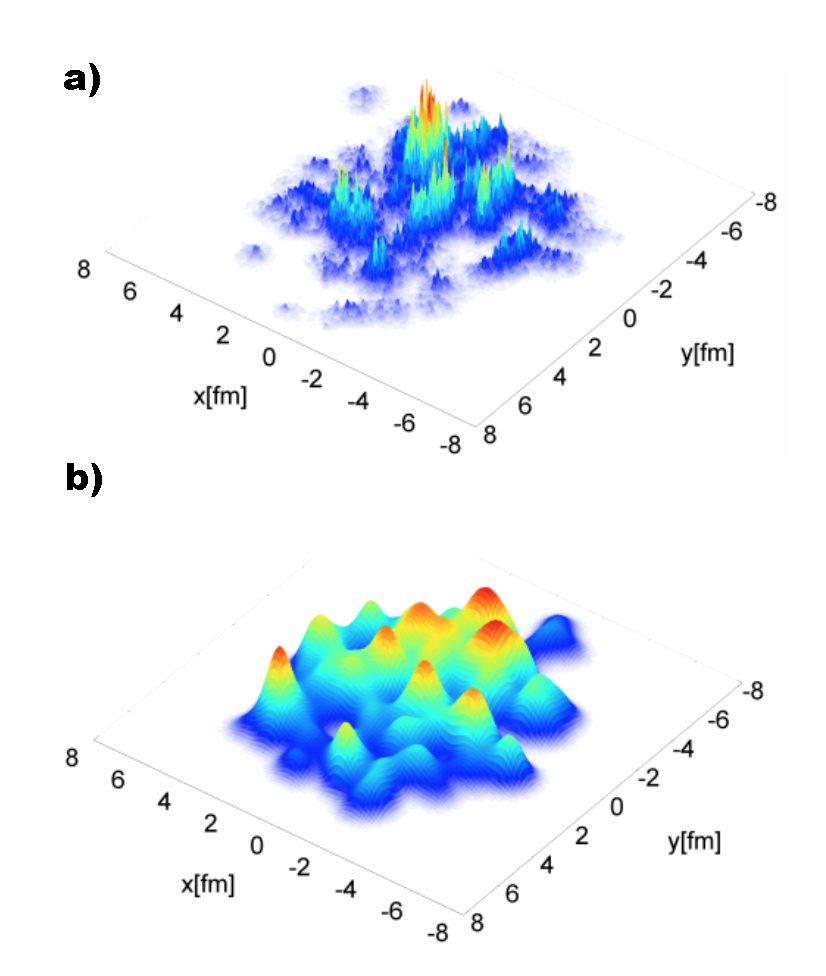
\includegraphics[width=0.45\linewidth]{figs/initial_conditions.png}
\caption{ a) IP-glasma. b) MC-KLN. c) MC-Glauber.}
\end{center}
\end{figure}
